\section{D. Irga B. Naufal Fakrhi (1174066)}
\subsection{Instalasi Map Server}
\begin{enumerate}
    \item Download aplikasi ms4w melalui website ms4w.com/download.html
    \hfill\break
    \begin{figure}[H]
		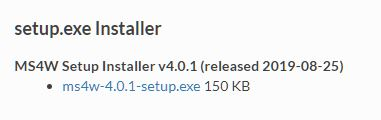
\includegraphics[width=4cm]{figures/tugas4/1174066/1.jpg}
		\centering
		\caption{Download MS4W}
    \end{figure}
    \hfill\break

    \item Setelah download buka aplikasi untuk melakukan instalasi.
    \item Pada saat instalasi pilih Full Install
\end{enumerate}

\subsection{Konfigurasi Map Server}
Ketika instalasi selesai, lakukan konfigurasi
\begin{enumerate}
  \item Buka folder ms4w pada c:/ms4w. Lalu masuk ke folder apache
  \hfill\break
    \begin{figure}[H]
		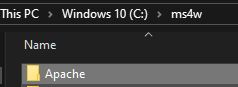
\includegraphics[width=4cm]{figures/tugas4/1174066/2.jpg}
		\centering
		\caption{Folder Apache}
    \end{figure}


  \item Masuk ke folder conf
  \hfill\break
    \begin{figure}[H]
		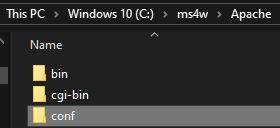
\includegraphics[width=4cm]{figures/tugas4/1174066/3.jpg}
		\centering
		\caption{Folder conf}
    \end{figure}

  \item Buka file httpd.conf menggunakan editor (notepad++) lalu cari tulisan Listen. Karena pada komputer saya port 80 digunakan oleh xampp maka saya ubah menjadi 2000.
  \hfill\break
    \begin{figure}[H]
		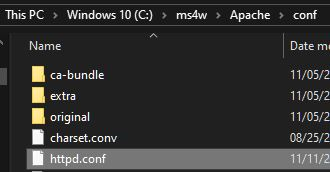
\includegraphics[width=4cm]{figures/tugas4/1174066/4.jpg}
		\centering
		\caption{File httpd.conf}
    \end{figure}

  \hfill\break
    \begin{figure}[H]
		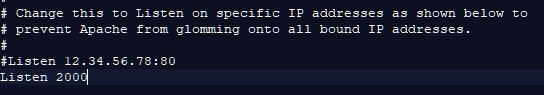
\includegraphics[width=4cm]{figures/tugas4/1174066/5.jpg}
		\centering
		\caption{Edit file httpd.conf}
    \end{figure}

  \item Kemudian kita restart service milik ms4w dengan cara, membuka task manager
  \hfill\break
    \begin{figure}[H]
		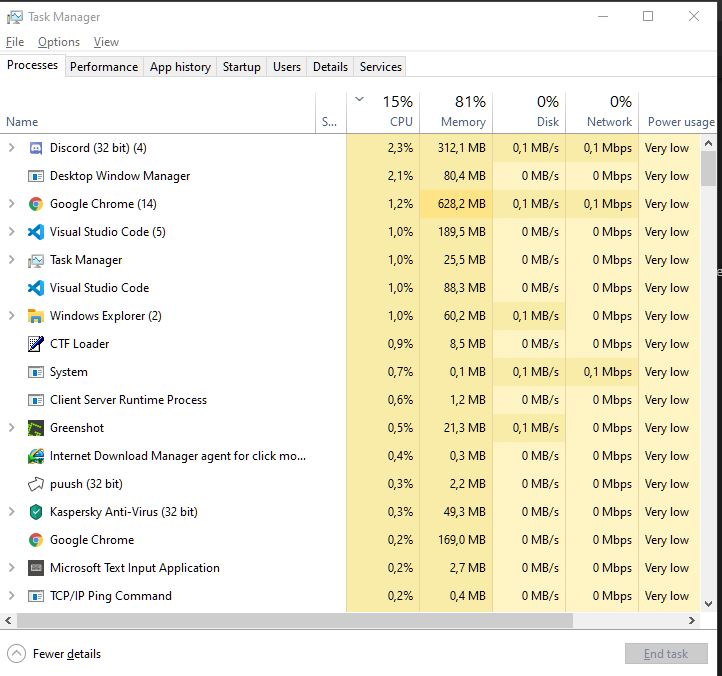
\includegraphics[width=4cm]{figures/tugas4/1174066/6.jpg}
		\centering
		\caption{Task Manager}
    \end{figure}

  \item Lalu pilih Services, cari ApacheMS4WWebServer
  \hfill\break
  \begin{figure}[H]
  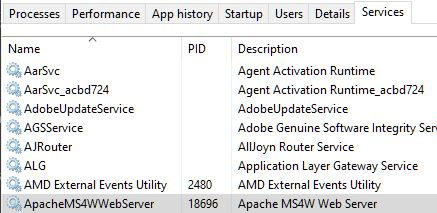
\includegraphics[width=4cm]{figures/tugas4/1174066/7.jpg}
  \centering
  \caption{Pilih tab service dan pilih ApacheMS4WWebServer}
  \end{figure}

  \item Klik kanan lalu tekan Restart
  \hfill\break
    \begin{figure}[H]
		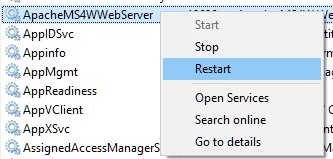
\includegraphics[width=4cm]{figures/tugas4/1174066/8.jpg}
		\centering
		\caption{Mengakses Halaman Service}
    \end{figure}
\end{enumerate}

\subsection{Link Youtube Instalasi MapServer}
https://youtu.be/I\_HfLAdagj4

\subsection{Instalasi MapProxy}
\begin{enumerate}
  \item Buka Command Prompt pada Windows
  \item Lalu ketikkan pip install MapProxy
  \hfill\break
  \begin{figure}[H]
  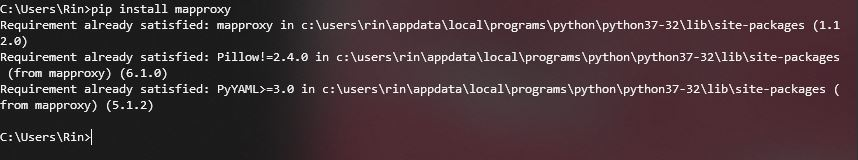
\includegraphics[width=4cm]{figures/tugas4/1174066/9.jpg}
  \centering
  \caption{Instalasi MapProxy}
  \end{figure}
\end{enumerate}

\subsection{Membuka map menggunakan MapProxy}
\begin{enumerate}
  \item Download / clone git dari https://github.com/awangga/gede
  \item Pastikan path menuju folder gede tidak ada spasi contohnya saya N:/gede-master
  \item Pada folder gede-master buat folder bernama tmp
  \hfill\break
  \begin{figure}[H]
  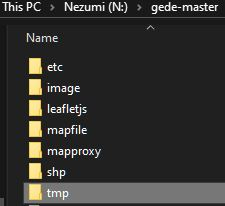
\includegraphics[width=4cm]{figures/tugas4/1174066/11.jpg}
  \centering
  \caption{Buat folder tmp}
  \end{figure}

  \item Setelah itu buka folder mapproxy lalu edit file agm.yaml
  \hfill\break
  \begin{figure}[H]
  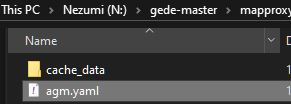
\includegraphics[width=4cm]{figures/tugas4/1174066/13.jpg}
  \centering
  \caption{File agm.yaml}
  \end{figure}

  \item Edit pada bagian sources lalu ada map, masukkan pathnya sesuai dengan dimana anda menyimpan file gede yang anda clone contohnya saya ada pada N:/gede-master/mapfile/mywms.map
  \hfill\break
  \begin{figure}[H]
  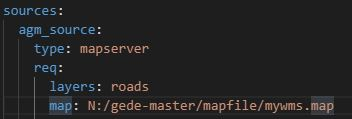
\includegraphics[width=4cm]{figures/tugas4/1174066/14.jpg}
  \centering
  \caption{Edit lokasi mymap.map}
  \end{figure}


  \item Lalu dibawahnya pada bagian binary masukkan lokasi instalasi ms4w anda, lalu tambahkan /Apache/cgi-bin/mapserv.exe, yang saya setelah diedit menjadi C:/ms4w/Apache/cgi-bin/mapserv.exe
  \hfill\break
  \begin{figure}[H]
  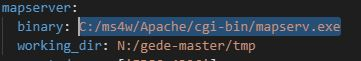
\includegraphics[width=4cm]{figures/tugas4/1174066/15.jpg}
  \centering
  \caption{Edit path binary mapserv}
  \end{figure}

  \item Setelah itu pada bagian working-dir masukkan path folder yang telah kita buat tadi, yang saya N:/gede-master/tmp
  \hfill\break
  \begin{figure}[H]
  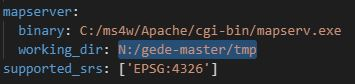
\includegraphics[width=4cm]{figures/tugas4/1174066/16.jpg}
  \centering
  \caption{Edit path working-dir}
  \end{figure}

  \item Setelah itu buka aplikasi MS4W-Shell
  \hfill\break
  \begin{figure}[H]
  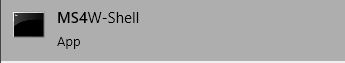
\includegraphics[width=4cm]{figures/tugas4/1174066/10.jpg}
  \centering
  \caption{Aplikasi MS4W-Shell}
  \end{figure}

  \item Setelah itu buka lokasi folder gede kita yang tadi telah di clone
  \hfill\break
  \begin{figure}[H]
  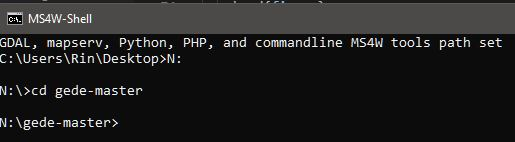
\includegraphics[width=4cm]{figures/tugas4/1174066/12.jpg}
  \centering
  \caption{Buka Folder gede}
  \end{figure}

  \item Setelah itu buka folder mapproxy yang ada pada folder gede
  \hfill\break
  \begin{figure}[H]
  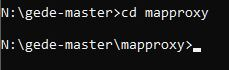
\includegraphics[width=4cm]{figures/tugas4/1174066/17.jpg}
  \centering
  \caption{Buka Folder mapproxy}
  \end{figure}

  \item setelah dibuka ketikkan "mapproxy-util serve-develop ./agm.yaml" pada ms4w-Shell untuk membuka aplikasi mapproxy
  \hfill\break
  \begin{figure}[H]
  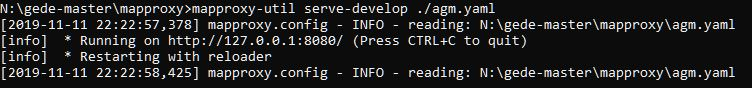
\includegraphics[width=4cm]{figures/tugas4/1174066/18.jpg}
  \centering
  \caption{Buka aplikasi mapproxy}
  \end{figure}
  
  \item Buka browser lalu ketikkan 127.0.0.1:8080
  \hfill\break
  \begin{figure}[H]
  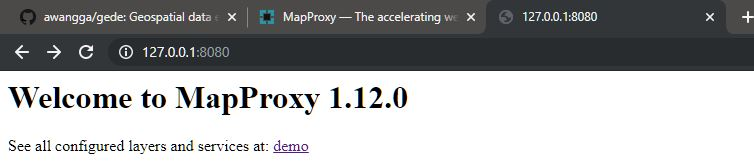
\includegraphics[width=4cm]{figures/tugas4/1174066/19.jpg}
  \centering
  \caption{Buka mapproxy pada browser}
  \end{figure}

  \item lalu klik demo untuk melihat map
  \item lalu klik png pada agm, maka mapproxy akan menampilkan map
  \hfill\break
  \begin{figure}[H]
  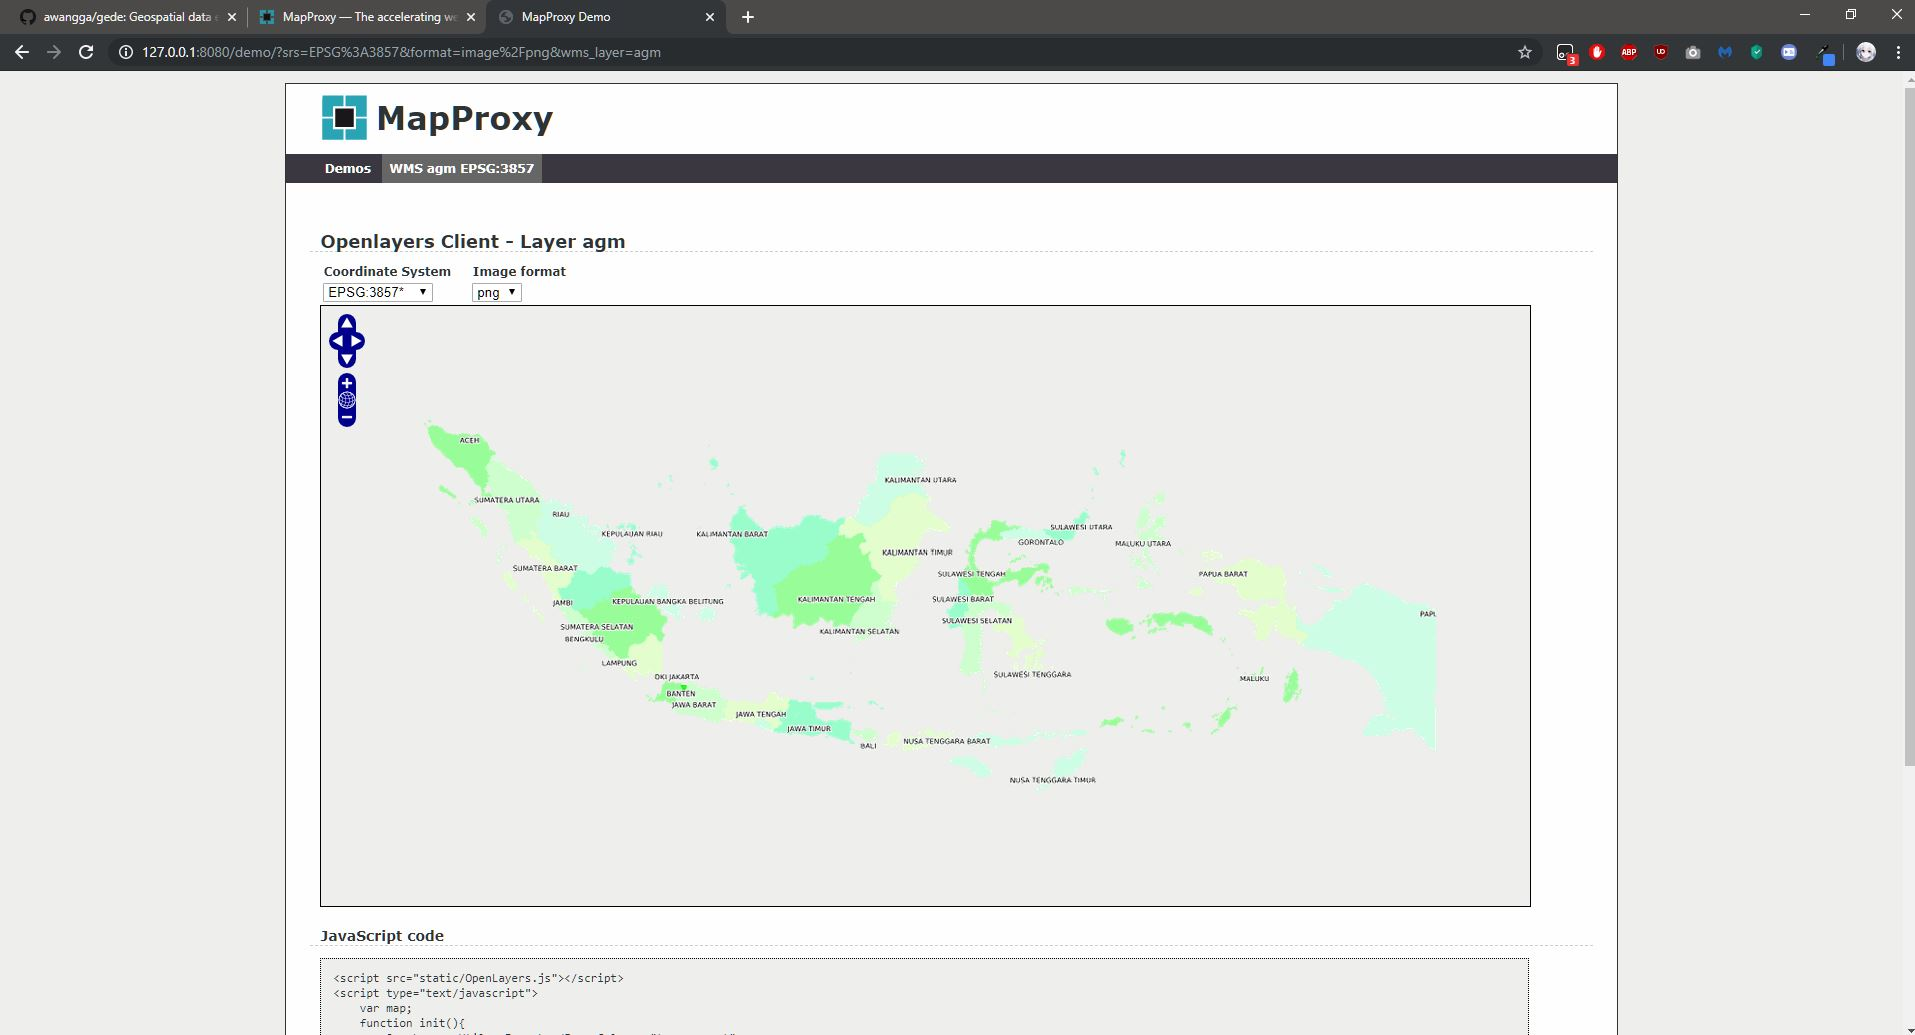
\includegraphics[width=4cm]{figures/tugas4/1174066/20.jpg}
  \centering
  \caption{MapProxy menampilkan map}
  \end{figure}

\end{enumerate}

\subsection{Link Youtube MapProxy dan Menjalankannya}
https://youtu.be/IF5aquR8Bb4
